\documentclass{article}
\usepackage{cmap}
\usepackage[T2A]{fontenc}
\usepackage[utf8]{inputenc}
\usepackage[english,russian]{babel}
\usepackage{setspace}
\usepackage{geometry}
\usepackage{graphicx}
\usepackage{amsfonts}
\graphicspath{{graphicslab3/}}
\DeclareGraphicsExtensions{.pdf, .png, .jpg, .fig}
\geometry{top=2cm}
\geometry{bottom=2cm}
\geometry{left=2cm} % отступ справа
\geometry{right=2cm} % отступ слева

\begin{document}
	\begin{center}
		\hfill \break
		\begin{center}
			\huge{Санкт-Петербургский политехнический университет\\
				Высшая школа прикладной математики\\
				и вычислительной физики, ФизМех}
		\end{center}
		\hfill \break
		\hfill \break
		\hfill \break
		\hfill \break
		\hfill \break
		\huge{Направление подготовки\\
			«Прикладная математика и информатика»}\\
		\hfill \break
		\hfill \break
		\hfill \break
		\hfill \break
		\hfill \break
		\hfill \break
		\fontsize{14pt}{14pt}\selectfont
		Отчет по лабораторной работе №3\\
		«Решение СЛАУ итерационными методами»\\
		\hfill \break
		\hfill \break
		\hfill \break
		\hfill \break
		\hfill \break
	\end{center}
	\hfill \break
	\hfill \break
	\fontsize{12pt}{12pt}\selectfont
	\begin{tabular}{cccc}
		\hspace{1cm}Выполнил студент гр. 5030102/00003 & {\hspace{3cm}} & & Петрошенко А.В. \\\\
		\hspace{-3cm}Преподаватель: &{\hspace{1cm}}& & {\hspace{1cm}} Курц В.В. \\\\
	\end{tabular}\\
	\hfill \break
	\hfill \break
	\hfill \break
	\hfill \break
	\hfill \break
	\hfill \break
	\begin{center} Санкт-Петербург\\ 
		2021\\
	\end{center}
	\thispagestyle{empty}
	\newpage
	\begin{center} \textbf{Формулировка задачи и ее формализация}\end{center}
	Большинство расчетных математических задач сводится к решению системы линейных алгебраических уравнений(далее СЛАУ). Существует 2 класса методов решения таких СЛАУ:
	\begin{enumerate}
		\item Прямые методы - методы, которые находят <<точные>> значения неизвестных за конечное число операций.
		\item Итерационные методы - методы, которые строят последовательность векторов, сходящихся к решению.
	\end{enumerate}
	В этой работе мы будем использовать итерационный метод.\\
	\\
	\underline{Постановка задачи:}\\
	Пусть дана система из $n$ линейных уравнений с $n$ неизвестными:
	\begin{center}
		$\sum\limits_{j = 1}^n a_{ij}x_j = b_i$, $i = 1, \ldots, n$
	\end{center}
	где $x_j$ - неизвестные, $a_{ij}$ - коэффициенты системы и $b_i$ - компоненты вектора правой части.\\
	В матричной форме: $$Ax = b$$
	где $A = (a_{ij}) \in \mathbb{R} ^{n \times n}$ - матрица коэффициентов, $b = (b_i) \in \mathbb{R}^n$ - вектор правой части и $x = (x_j) \in \mathbb{R}^n$ - вектор неизвестных.\\
	Требуется найти решение с точностью $\epsilon$, то есть $||x^k - x^*|| < \epsilon$\\
	В данной работе будет реализован и описан Градиентный метод.\\
	\begin{center} \textbf{Алгоритм метода и условия его применимости}\end{center}
	Определим квадратичную форму: $$F(y) = (Ay, y) - 2(b, y)$$
	Каждое следующее приближение будем получать, двигаясь в направлении противоположном градиенту квадратичной формы, введенной выше: $$x^{k+1} = x^k - \alpha_k \nabla F(x^k), \alpha_k > 0$$
	$$\nabla F(x^k) = 2(Ax^k - b) = g^k$$
	Причем $\alpha_k$ нужно выбирать так, чтобы $F(x^k) \to min$\\
	Из теоремы о том, что $x^*$ является решением системы $\Leftrightarrow$ $x^*$ сообщает минимум квадратичной формы $F(y)$ мы знаем, что: $$\phi '(\alpha_k) = 0 \Rightarrow \alpha_k = \frac{(g^k, g^k)}{2(Ag^k, g^k)}$$\\
	Останавливаться будем по условию: $$||x^{k+1} - x^*||_{H_A} \leq \frac{M}{1-M}||x^{k+1} - x^k||_{H_A} \Leftrightarrow ||x^{k+1} - x^k||_{H_A} \geq \frac{1-M}{M} \epsilon$$\\
	Данное условие было получено из неравенства $||e^{k+1}||_{H_A} \leq M||e^k||_{H_A}$, где $M = \frac{cond(A) - 1}{cond(A) + 1}$\\
	Также стоит добавить, что $||v||_{H_A} = (Av, v)$\\
	\underline{Условия применимости:}\\
	Квадратная матрица $A$ должна быть симметричной и положительно определенной.
	\begin{center} \textbf{Предварительный анализ задачи}\end{center}
	\underline{Построение матрицы:}\\
	Любую симметричную матрицу можно разложить в виде $A = QDQ^T$, где матрица $Q$ - это ортогональная матрица, а $D$ - диагональная матрица, на диагонали которой стоят только положительные числа. Т.к. они являются собственными числами матрицы $A$, то из данного разложения следует, что она будет и положительно определенной.
	\begin{center} \textbf{Тестовый пример для задач малой размерности}\end{center}
	Возьмем ортогональную матрицу: $Q = \left(
	\begin{array}{ccc}
		-0.9812  &  0.1729  &  0.0854\\
		-0.1762  & -0.6237  & -0.7615\\
		-0.0784  & -0.7623  &  0.6425
	\end{array}
	\right)$, $D = \left(
	\begin{array}{ccc}
		1  &  0  &  0\\
		0  &  2  &  0\\
		0  &  0  &  3
	\end{array}
	\right)$\\
	\\
	Тогда $A = \left(
	\begin{array}{ccc}
		 1.0444  & -0.2379  & -0.0221\\
		-0.2379  &  2.5487  & -0.5031\\
		-0.0221  & -0.5031  &  2.4068
	\end{array}
	\right)$\\
	\\
	\\
	Рассмотрим СЛАУ:
	$\left\{
	\begin{array}{ccc}
		 1.0444x_1  -  0.2379x_2  -  0.0221x_3 = 0.7844\\
		-0.2379x_1  +  2.5487x_2  -  0.5031x_3 = 1.8077\\
		-0.0221x_1  -  0.5031x_2  +  2.4068x_3 = 1.8816
	\end{array}
	\right.$\\
	Ее точное решение: $x^* = \left(
	\begin{array}{c}
		1\\
		1\\
		1
	\end{array}
	\right)$\\
	Возьмем $x^0 = \left(
	\begin{array}{c}
		0\\
		0\\
		0
	\end{array}
	\right)$ и найдем решение с точностью $\epsilon = 0.1$:\\
	Комментарий: Для сокращения вычислений, сократим 2-ки в формулах  $g^k$ и $\alpha_k$\\
	\\
	Из матрицы $D$ получаем, что $cond(A) = 3 \Rightarrow M = 0.5 \Rightarrow \frac{1-M}{M} = 1$
	\begin{enumerate}
		\item $g^0 = -b = \left(\begin{array}{c}
			-0.7844\\
			-1.8077\\
			-1.8816
		\end{array}\right)$\\
	$\alpha_0 = 0.5569$\\
	$x^1 = x^0-\alpha_0 g^0 = \left(\begin{array}{c}
		0.4368\\
		1.0067\\
		1.0479
	\end{array}\right)$\\
	$||x^1 - x^0||_{H_A} = 2.0333 \geq 0.1$
	\item $g^1 = \left(\begin{array}{c}
		-0.5908\\
		 0.1270\\
		 0.1243
	\end{array}\right)$\\
	$\alpha_1 = 0.8170$\\
	$x^2 = \left(\begin{array}{c}
		0.9195\\
		0.9029\\
		0.9463
	\end{array}\right)$\\
	$||x^2 - x^1||_{H_A} = 0.5577 \geq 0.1$
	\item $g^2 = \left(\begin{array}{c}
		-0.0598\\
		-0.2012\\
		-0.0786
	\end{array}\right)$\\
	$\alpha_2 = 0.5026$\\
	$x^3 = \left(\begin{array}{c}
		0.9496\\
		1.0041\\
		0.9858
	\end{array}\right)$\\
	$||x^3 - x^2||_{H_A} = 0.1589 \geq 0.1$
	\item $g^3 = \left(\begin{array}{c}
		-0.0533\\
		 0.0295\\
		-0.0351
	\end{array}\right)$\\
	$\alpha_3 = 0.5015$\\
	$x^4 = \left(\begin{array}{c}
		0.9763\\
		0.9893\\
		1.0034
	\end{array}\right)$\\
	$||x^4 - x^3||_{H_A} = 0.0498 < 0.1$
	\end{enumerate}
	Мы получили ответ с заданной точностью за 4 итерации, не считая начальное прриближение.
	\begin{center} \textbf{Контрольные тесты}\end{center}
	\begin{enumerate}
		\item Создадим 4 матрицы 10$\times$10 с числами обусловленности $10, 10^2, 10^3, 10^4$ и найдем их решения с помощью градиентного метода с точностью $\epsilon = 10^{-10}$
		\item Создадим 101 матрицу, меняя ее ранг с 1000$\times$1000 до 2000$\times$2000 с шагом в 10. Найдем решение с помощью метода Холецкого, получим ошибку и затем найдем решение с помощью градиентного метода с точностью, равной полученной ошибке, но умноженной на 10 для решения проблемы с машинным эпсилон. Для каждого из методов будем засекать время их выполнения, после чего сравним их.
	\end{enumerate}
	\begin{center} \textbf{Модульная структура программы}\end{center}
	\verb|typedef struct{|\\
		\hspace*{1cm} \verb|vector<vector<double>> A;|\\
		\hspace*{1cm} \verb|int rang;|\\
		\verb|}matrix_t;|\\
	- структура данных, имеющая 2 поля: двумерный массив для значений матрицы и целое число для хранения ранга матрицы.\\
	\\
	\verb|int GetNum(const char* filename)| - функция для получения одного числа из файла. Использовалась для получения из файла ранга матриц и их количества.\\
	\\
	\verb|matrix_t ImportMatrix(vector<double> str, int rang)|\\
	\verb|vector<double> ImportRightPart(vector<double> str, int rang)|\\ 
	Функции, преобразующие данные, полученные из файла в удобный вид(матрицу или вектор).\\
	\\
	\verb|matrix_t Zero(int rang)|\\
	\verb|matrix_t Transpose(matrix_t matrix)|\\
	\verb|matrix_t CholFactorization(matrix_t matrix)|\\
	\verb|vector<double> FindY(matrix_t matrix, vector<double> b)|\\
	\verb|vector<double> FindX(matrix_t matrix, vector<double> y)|\\
	Реализация метода Холецкого(функции описаны в предыдущем отчете)\\
	\\
	\verb|vector<double> RandomVector(int size)|\\
	\verb|vector<double> VectorSubstract(vector<double> vec1, vector<double> vec2)|\\
	\verb|vector<double> MatrixMulVector(matrix_t matrix, vector<double> vec)|\\
	\verb|vector<double> VectorMulNumber(vector<double> vec, double num)|\\
	\verb|double ScalarProduct(vector<double> vec1, vector<double> vec2)|\\
	\verb|double Norm(vector<double> vec)|\\
	\verb|double EnergyNorm(vector<double> vec, matrix_t A)|\\
	\verb|vector<double> Gradient(matrix_t A, vector<double> x, vector<double> b)|\\
	\verb|double AlphaCoefficient(vector<double> g, matrix_t A)|\\
	Вспомогательные функции для градиентного метода(названия функций передают их смысл)\\
	\\
	\verb|vector<vector<double>> GradientMethod(matrix_t A, vector<double> b, double|\\ \verb|cond, double eps)|\\
	Реализация градиентного метода\\
	\\
	\verb|void OutputVector(vector<double> vec, const char* filename)|\\
	\verb|void OutputMatrix(matrix_t matrix, const char* filename)|\\
	Функции записи нужных для дальнейшего анализа данных в файл.
	\begin{center} \textbf{Численный анализ}\end{center}
	$\triangleright$ \underline{Точность:}\\
	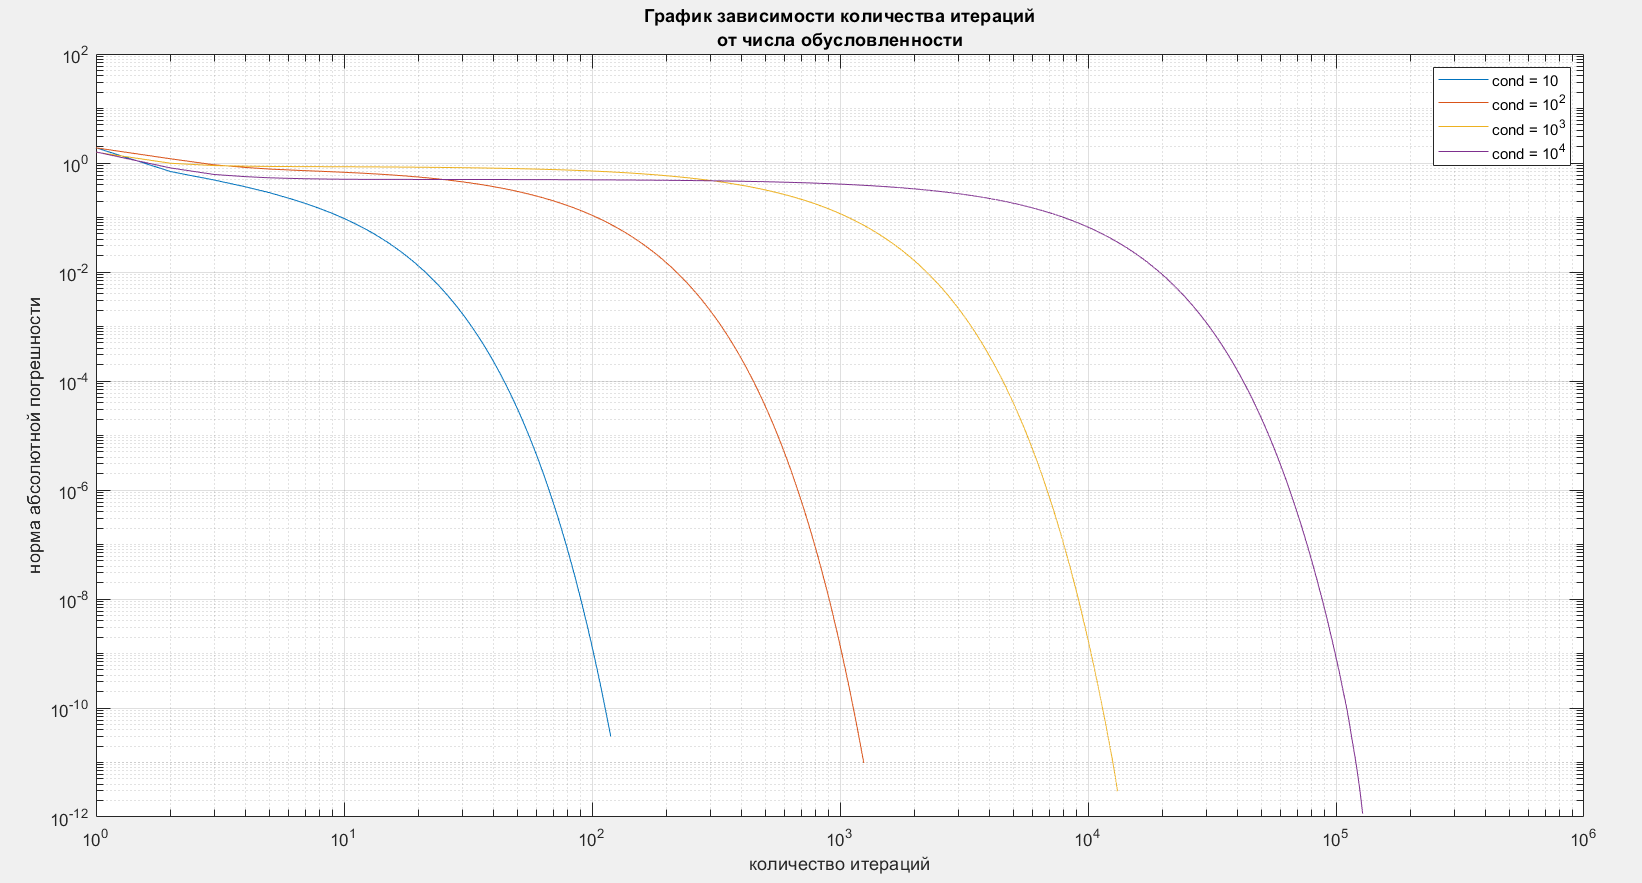
\includegraphics[scale = 0.4]{Итерации}\\
	Из графика мы видим, что поставленная точность достигается во всех случаях($\epsilon = 10^{-10}$). Видна зависимость от числа обусловленности: чем оно больше, тем дольше сходится метод, но и тем точнее решение.\\
	$\triangleright$ \underline{Объем вычислений:}\\
	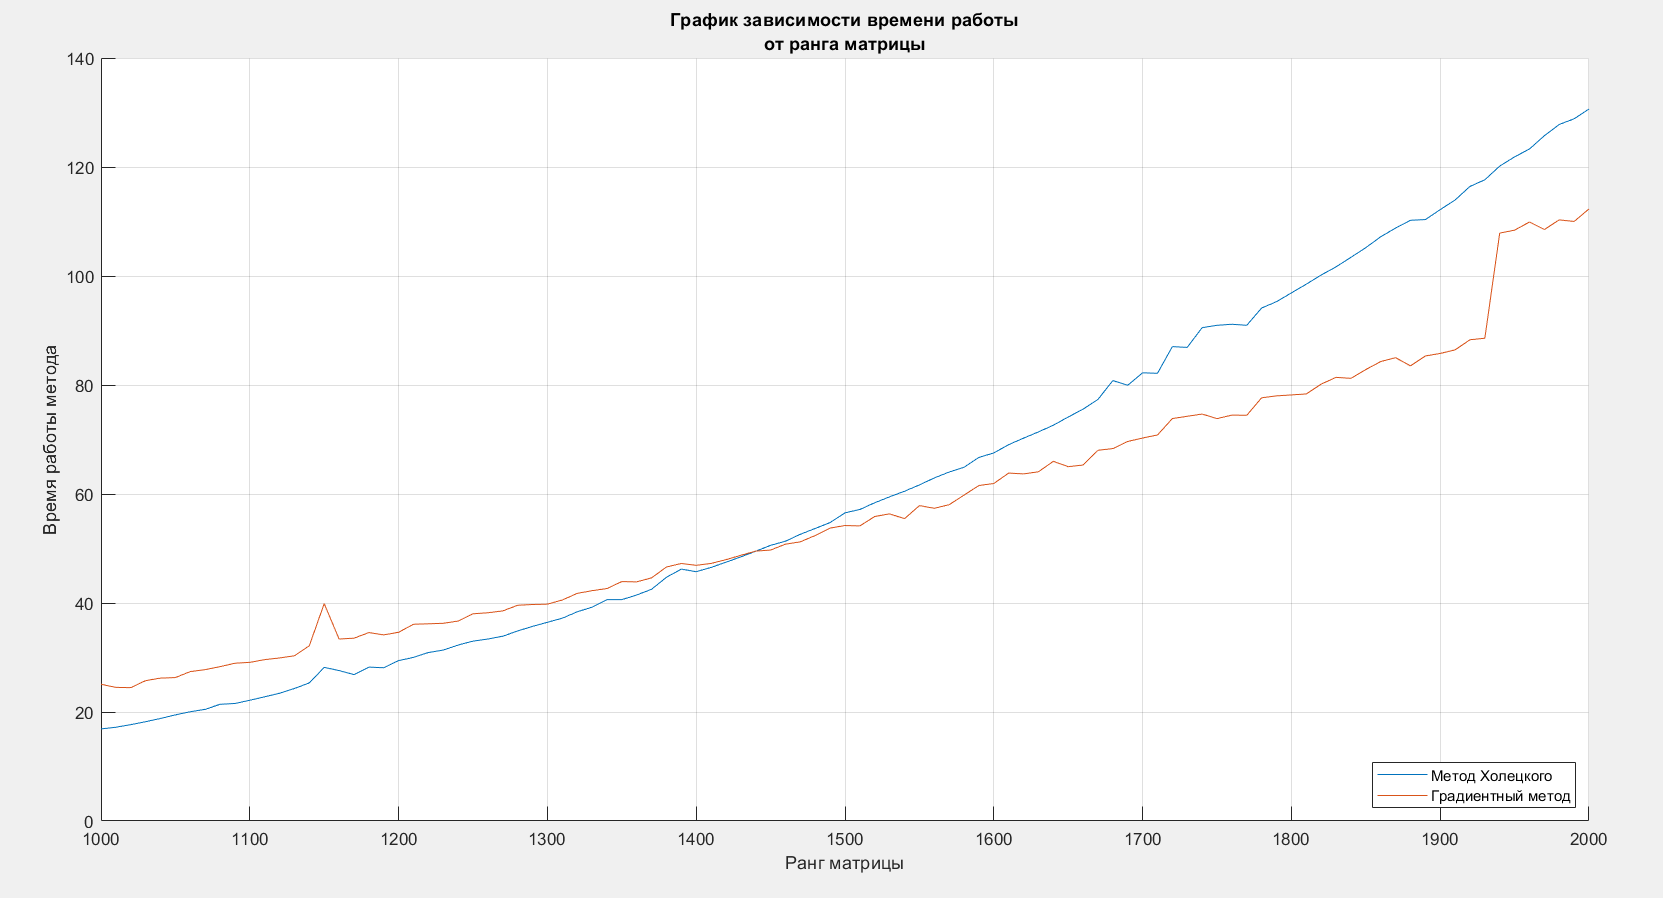
\includegraphics[scale = 0.4]{Время}\\
	На графике явно видно, что, начиная примерно с матрицы 1500$\times$1500 метод Холецкого становится дольше градиентного метода, что связано с различием в принципах работы прямых и итерационных методов. Делаем вывод, что итерационные методы лучше применять на больших матрицах, когда прямые на матрицах меньшей размерности.
	\newpage
	\begin{center} \textbf{Общие выводы:}\end{center}
	В данной лабораторной работе мы научились находить решения СЛАУ градиентным методом. Проанализировали зависимость работы метода от числа обусловленности матрицы и сравнили время работы прямого метода(метода Холецкого) и итерационного(градиентного метода). Различие в принципах работы прямых и итерационных методов состоит в том, что прямые методы приводят исходную матрицу к удобному для нахождения решения виду, на что тратят много времени при больших размерах матрицы, когда итерационные методы, в свою очередь, не меняют исходную матрицу, а сразу начинают приближение к решению, за счет чего и выигрывают на больших матрицах.
\end{document}